\newcommand{\cmdname}[1]{\cmnd{#1}{#1}}
\newcommand{\ilinput}[1]{\ttout{#1}}
\newcommand{\crsname}{COMP10120}
\newcommand{\Dcrsname}{???}
\newcommand{\crsnamelc}{comp10120}
\newcommand{\return}{\relax}

This section to practice your command line skills and prepare for next week

\subsection{Creating a directory structure}

You're now going to use the \cmdname{mkdir} (``make directory'') command
to create some directories. Type

\begin{ttoutenv}
  mkdir \crsname\return
\end{ttoutenv}
%
Check that this directory has indeed appeared using \cmdname{ls}.

It's important that directories we ask you to make for your work have
exactly the names we specify. Unix will let you use any names you
like, but we have to impose conventions for administrative reasons.

If you made a mistake, e.g. \fname{\crsnamelc} instead of \fname{\crsname},
you can remove the directory while it is still empty with the
\cmdname{rmdir} command: e.g.
%
\begin{ttoutenv}
  rmdir \crsnamelc\return
\end{ttoutenv}
%
And then try to make it correctly.

The \cmdname{cd} (``change directory'') command allows you to move around
the tree by changing your current working directory. Type
%
\begin{ttoutenv}
  cd \crsname\return
\end{ttoutenv}
%
to make \crsname{} your working directory. Check that you have changed
current directory using \cmnd{pwd}{pwd}.

  
Now make directories for each of the \crsname{} exercises.

\begin{ttoutenv}
  mkdir ex1 ex2 ex3 \return
\end{ttoutenv}
%  mkdir ex1 ex2 ex3 ex4 \return
%
Recall that the \cmdname{cd} command on its own takes you back to your home
directory, wherever you may be when you invoke it.  Try this out by
typing

\begin{ttoutenv}
  cd \return
\end{ttoutenv}

Check that you are now in your home directory.

Your directory structure should now look something like this
%\begin{firstonly}
     \begin{center}
       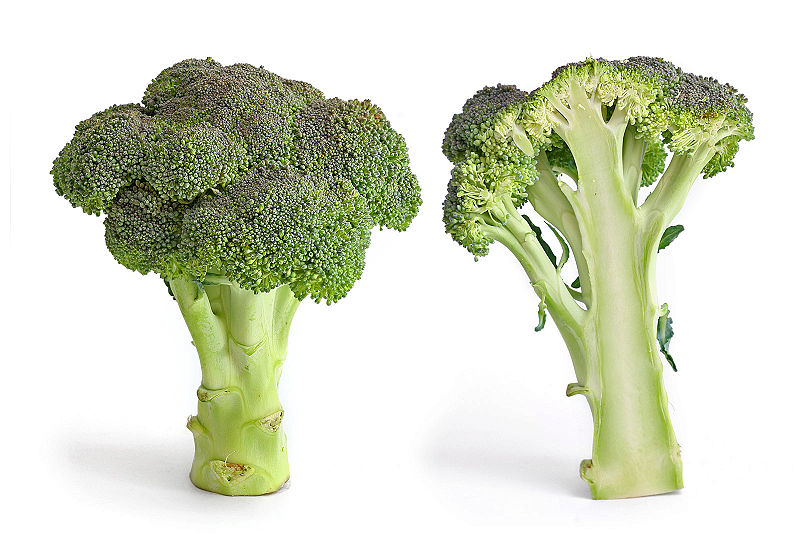
\includegraphics[width=0.4\textwidth]{images/broccoli} %ps/dirs.eps}
     \end{center}
%\end{firstonly}

%\begin{msconly}
%     \begin{center}
%       \includegraphics[width=0.4\textwidth]{ps/dirs-msc.eps}
%     \end{center}
%\end{msconly}
     
The easiest way to check this is to use (from your home directory)
\cmdname{ls} with the \ttout{-R} flag. This shows the whole tree
below your current working directory (\ttout{-R} is short for
\wikipedia{Recursion}{``recursively'}'  -- look up the word in a dictionary, or wait until later for a
 definition!).

\begin{ttoutenv}
\$ ls -R 
\end{ttoutenv}
%

  Now you should make a directory for the COMP16121 course unit
  %(or COMP16920
  %if you
%  are an ABIS student) with
  %are a CSE student)
  with
  sub-directories for each of the 10 exercises associated with that
  course. You \emph{must} use the same convention as above:
  capital ``COMP16121'' and lower case ``ex1'', etc..

You must get your directory structure right before continuing -- ask a
member of the lab staff to check it at this point.


\subsection{Copying, moving, and removing files}

This subsection re-introduces three commands used for copying, moving and
removing files. We first describe each command and then invite you to
practice using them.

\noindent The \cmdname{cp} (copy) command has two forms.

\begin{note}
  fix <file> [file] notation
\end{note}

The first general form is
\begin{ttoutenv}
  cp <file> <file> \return
\end{ttoutenv}

For example

\begin{ttoutenv}
  cp file1 file2 \return
\end{ttoutenv}
%
makes a copy of the file \fname{file1} and calls it \fname{file2}.  If
a file called file2 already exists, \emph{the existing \fname{file2} will be  overwritten
with a copy of \fname{file1} and lost without warning}.

The second form is slightly different:
\begin{ttoutenv}
  cp <file(s)> <directory>
\end{ttoutenv}
%
For example

\begin{ttoutenv}
  cp file1 file2 file3 dirname \return
\end{ttoutenv}

This copies the files \fname{file1}, \fname{file2}, \fname{file3} into
the directory \fname{dirname}, again overwriting any files already
there with the same names.

The command \cmdname{rm} (remove) is used to delete files.
\begin{ttoutenv}
  rm <file(s)>
\end{ttoutenv}
%
throws away the specified files -- always take great care when using
\cmdname{rm}, it is not reversible.

The \cmdname{mv} (move) command is similar to \cmdname{cp}, but it just moves
the files rather than makes copies. Again we have the two forms
\begin{ttoutenv}
  mv <file1> <file2> \return
\end{ttoutenv}
and
\begin{ttoutenv}
  mv <file(s)> <directory> \return
\end{ttoutenv}

The effect is like a copying followed by removing the sources of the copy,
except it is more efficient than that (most of the time).
For example
\begin{ttoutenv}
  mv file1 file2 \return
\end{ttoutenv}
is like doing
\begin{ttoutenv}
  cp file1 file2 \return
  rm file1
\end{ttoutenv}
and
\begin{ttoutenv}
  mv file1 file2 file3 dirname \return
\end{ttoutenv}
is like doing
\begin{ttoutenv}
  cp file1 file2 file3 dirname \return
  rm file1 file2 file3
\end{ttoutenv}

Before continuing, answer this question and check your answer with a
member of staff: how do you \emph{rename} a file in Unix? Don't guess -- you
know the answer, unless you are going too fast.

Now for some practice. Go to your home directory
%
\begin{ttoutenv}
  cd \return
\end{ttoutenv}
%
and copy the file called \fname{lightbulbs} in the \fname{\Dcrsname}
directory to your current working directory:

\begin{note}
Tell them about .  
\end{note}

\begin{ttoutenv}
  cp \Dcrsname/lightbulbs .  \return
\end{ttoutenv}
%
Note that \ilinput{\Dcrsname} must be in uppercase and the full stop is
essential.  If you now do an \cmdname{ls}, you should see that the
file called \fname{lightbulbs} has appeared in your directory:

\begin{ttoutenv}
  ls \return
\end{ttoutenv}

If no file called \fname{lightbulbs} has appeared, the following will
probably provide an explanation. If it did appear, read this anyway, just to
check that you understand what you did right!

The \cmdname{cp} command needs two arguments. In this case, the file
you are copying is \fname{\Dcrsname/lightbulbs}, and the directory
you are copying it to is ``.'' (that is, your current working
directory -- remember every directory has a reference to itself within
it, called `.'?). If you missed out the dot, or mis-spelt
\fname{\Dcrsname/lightbulbs}, or missed out one of the spaces, it
won't have worked. In particular, you may well have got a
``friendly'', helpful error message like:
%
%  Usage: cp [-ip] f1 f2; or: cp [-irp] f1 ... fn d2
\begin{ttoutenv}
  cp: missing destination file
  Try `cp --help' for more information.
\end{ttoutenv}
%
or
\begin{ttoutenv}
  cp: /opt/info/courses/\crsname/lightblurbs: No such file or directory
\end{ttoutenv}
or
\begin{ttoutenv}
  cp: \crsname/lightbulbs: No such file or directory
\end{ttoutenv}
%
If you get the first message, it means you used the command with the
wrong number of arguments, and nothing will have happened.
The others are examples of what you might see if you mistype the first
argument. If you do get an error message you need to give the command again,
correctly, to copy the lightbulbs file across.

So you now have a copy of the file, but, it's in your home directory.
You'll have to get into the habit of \emph{not} having all your files
in your home directory, otherwise you will quickly have an enormous list
that will take you ages to find anything in. The use of subdirectories
provides a solution to this problem, which is why you created some
earlier. Moving this file to the ``correct'' place gives you a chance
to practice the \cmdname{mv} command.

Move the file \fname{lightbulbs} to your \fname{\crsname/ex2} directory.

Notice that \fname{\crsname} is \emph{your\/} \crsname{} directory, while
\fname{\Dcrsname} is (an abbreviation for) \emph{our\/} \crsname{}
directory, from which you can read things but cannot write to.

Now go to your \fname{\crsname/ex2} directory and check that the file
has arrived there.

To make sure you understand \cmdname{cp}, \cmdname{mv}, and
\cmdname{rm}, go through the following sequence (in your
\fname{\crsname/ex2} directory), checking the result by looking at the
output from \cmdname{ls} at each stage

\begin{ttoutenv}
  cp lightbulbs bulb1 \return
  ls \return
  cp lightbulbs bulb2 \return
  ls \return
  mv bulb1 bulb3 \return
  ls \return
  cp bulb3 bulb4 \return
  ls \return
  rm bulb2 \return
  ls \return
  rm bulb1 \return
  ls \return
\end{ttoutenv}
Why does \ilinput{rm bulb1} behave differently to \ilinput{rm bulb2}?

\subsection{Wild cards}
An asterisk in a filename is a \textbf{wild card} which matches any sequence of
zero or more characters, so for instance, if you were to type (don't
actually do it!)
%
\begin{ttoutenv}
  rm *fred*\return
\end{ttoutenv}
%
then all files in the current directory whose names contain the string
``fred'' would be removed.

Try the effect of
%
\begin{ttoutenv}
  ls bulb*\return
\end{ttoutenv}
%
and
%
\begin{ttoutenv}
  ls *bulb*\return
\end{ttoutenv}

Now try
%
\begin{ttoutenv}
  echo *bulb*\return
\end{ttoutenv}
%
Are you surprised by the result?

One exception to the above rule is provided by the dotfiles; i.e. those
whose names begin with ``.''. The asterisk will not match a
``.'' at the start of a file name. To see what this means try the
following
\begin{ttoutenv}
  cd \return 
  ls *xinit* \return
\end{ttoutenv}
%
and
%
\begin{ttoutenv}
  ls .*xinit*\return
\end{ttoutenv}
and see the different output.

\subsection{Quotas}
The command

\begin{ttoutenv}
  quota\return
\end{ttoutenv}

shows you what your file store quota is, and how much of it you are
actually using. This is only of academic interest now, but may become
very important later in the year! You may find that you are unable to
save files, or even receive mail, if you use more than your quota of
file store. It is important that, if this happens, you do something
about it immediately.
%Some tips as to what do if this happens can be
%found on the \htmladdnormallink{local Software Links web
%%  page}{http://www.cs.manchester.ac.uk/software/}.
%  page}{\localSoftware}.

 
\subsection{Putting commands together}
Before you forget that you're in your home directory, change directory back to
your \crsname/ex2.

One of the simplest (and most useful) of Unix commands is
\cmdname{cat}. This command has many uses, one of which is to
con\textbf{cat}enate a list of files given as arguments and display
their contents on the screen. For example
\begin{ttoutenv}
cat file1 file2 file3 \return
\end{ttoutenv}
would display the contents of the three files \fname{file1},
\fname{file2} and \fname{file3}.
The output from \cmdname{cat} goes to what is known as the
\textbf{standard output} (in this case the screen).

If you type  
\begin{ttoutenv}
cat \return
\end{ttoutenv}
nothing will happen because you haven't given a file to \cmdname{cat}.
When run like this, it takes its data from the \textbf{standard input},
which in this case is the keyboard, and copies it to the standard
output. Anything that you now type will be taken as input by
\cmdname{cat}, and will be output once each line of the input is
complete. In Unix, end of input is signalled by \ilinput{<Ctrl>d}.
(Recall that typing \ilinput{<Ctrl>d} in your login shell will log you
out -- you have told the shell to expect no more input.) So, after
typing \cmdname{cat} above, if you type (we will omit the \return's
from now on, we hope you've got the message)
\begin{ttoutenv}
This is
some 
text for cat to 
digest
<Ctrl>d
\end{ttoutenv}
you will see the input replicated on the output (interleaved line by
line with the input). The first copy is the echo of what you typed as
you typed it, the second copy is output from \cmdname{cat}. This may
not seem very useful, and you wouldn't actually use it just like that,
%(An example where you really would have cat do just this is a bit too
%complicated to show here!) 
%We've merely asked you to do that to
but it illustrates the point that \cmdname{cat} takes its input and copies it
to its output. Using this basic idea we can do various things to
change where the input comes from and where the output goes.

\begin{ttoutenv}
cat > fred1
\end{ttoutenv}
will cause the standard output to be directed to the file \fname{fred1}
in the working directory (the input still comes from the keyboard and
will need a \ilinput{<Ctrl>d} to terminate it. Try creating a file
\cmdname{fred1} using this technique, and then check its contents.

\begin{ttoutenv}
cat < fred1 
\end{ttoutenv}
will take the standard input from the file \fname{fred1}
in the working directory and make it appear on the screen. This has
exactly the same effect as 
\begin{ttoutenv}
cat fred1 
\end{ttoutenv}

You can, of course, use < and > together, as in
\begin{ttoutenv}
cat < fred1 > fred2
\end{ttoutenv}
which will copy the contents of the first file to the second. Try this and
check the results.

We can, of course, do this type of redirection with other
commands. For example, if we want to save the result of listing a
directory's contents into a file we just type something like
\begin{ttoutenv}
ls -l > fred1
\end{ttoutenv}
(this overwrites the previous contents of \fname{fred1} without
warning, so be careful of this kind of use).

One of the other things that \cmdname{cat} can do is to put line
numbers on its output. It does this if you use the \ilinput{-n}
flag. Try
\begin{ttoutenv}
cat -n fred1
\end{ttoutenv}
Now suppose, for the sake of argument, we wanted to have a listing of the
names of the
files in the current directory, with each line numbered, and the result
saved in a file \cmdname{fred3}. You have just been given all the
information you need to do this -- so, how would you do it? Do it now.

Unless you've met Unix before, you probably did something like this
\begin{ttoutenv}
ls > tmpfile 
cat -n tmpfile > fred3
\end{ttoutenv}
Or if you didn't then try it now and examine the contents of
\fname{fred3}. The file \fname{tmpfile} can now be thrown away using
\ilinput{rm tmpfile}.

It's a shame we had to use an extra, temporary, file. Could we avoid
having to? Why do you think the following would not work?
\begin{ttoutenv}
ls > fred3 
cat -n fred3 > fred3
\end{ttoutenv}

A better way of doing the task, which avoids the use of a temporary file
is by use of a powerful Unix feature called the \textbf{pipe}. We just type
\begin{ttoutenv}
ls | cat -n > fred3
\end{ttoutenv}
The \textbf{pipe} symbol \verb+|+ indicates that the \textbf{standard
output} of the first command is to be \textbf{piped} into the
\textbf{standard input} of the second command, so no intermediate file
is needed.

We can construct another (slightly artificial) pipeline example using
just \cmdname{cat}.

\begin{ttoutenv}
cat < fred1 | cat > fred2
\end{ttoutenv}
The first \cmdname{cat} takes its input from
\fname{fred1} and sends its output into the pipe. The second
\cmdname{cat} takes its input from the pipe (i.e. the output from the
first \cmdname{cat}) and sends its output to \cmdname{fred2}. (How many
other ways can you think of to do this?)  This isn't a frightfully sensible
thing to do, but it does illustrate the principle of piping (long
pipelines of commands may be constructed), and more realistic examples
will appear in the exercises.

Standard output sent to the screen may come so fast that it
disappears off the top before you have had a chance to read it.
There are three ways around this problem.
\begin{itemize}
\item Using foresight, pipe the output into the command \cmdname{more}
  or \cmdname{less}
  which arranges to stop after each page full. For example,
  \begin{ttoutenv}
  ls -la | less
  \end{ttoutenv}
  would be a wise precaution if the current working directory held
  more than a screen full of entries. When \cmdname{less} has shown you the
  first screen full, press \ilinput{<Space>} to see the next screen full,
  or \return to see just the next line.
\item 
  Without foresight, the output will rush past you at a great rate
  of knots. Press \ilinput{<Ctrl>s} to stop it dead in its tracks
  (and \ilinput{<Ctrl>q} to set it off again).
  In practice this isn't much use nowadays -- in most cases the computer is
  just too fast for the Human to press the keys at the right time.
\end{itemize}
%Now would be a good time to remove all those junk files like
%\fname{fred1} etc.
%\subsection{Newsgroups}\label{news}
%A useful facility to explore is the Usenet News system. It comprises
%literally thousands of groups on every conceivable topic to which you
%can subscribe and contribute.
%
%A convenient way to browse newsgroups is to use Mozilla in a similar
%way to the reading of mail. (A BIT MORE DESCRIPTION NEEDED HERE)
%
%The newsgroup man.cs.undergrad.first is used for messages to all first
%year students. It is important that you read information from this
%group regularly.
%
%When you are fed up with a group click on \ilinput{quit}, and when you
%have finished with news click on \ilinput{quit} from the list of
%newsgroups.
%
%Test question: What does the first unread message on
%man.cs.undergrad.first say?

\subsection{Printing text files}

The command \cmdname{lpr} can be used to send files to a printer. In its
simplest form, you simply run:
%
\begin{ttoutenv}
  lpr file1 file2
\end{ttoutenv}
%
to print the given files. You could use it now to print out the
\fname{lightbulbs} file, but that file is quite big and we don't want to waste
a lot of paper. So please don't! However, it would be nice to practice using
\cmdname{lpr}. So, you shall print out just the first 50 lines of it. Look at
the man page for \cmdname{lpr} and discover what it does if no file names are
given. Now look at the man page for the command \cmdname{head} and figure out
how to make it output the first 50 lines of the file \fname{lightbulbs}.
Experiment with this to make the 50 lines appear on your screen. From what you
have already learnt, you should know how to check there are exactly 50 lines
using the counting option of \cmdname{cat}. Now send the 50 lines to the
printer -- without using an temporary file. Go and collect your print output
-- ask for directions to where the printer is.
%
% head -50 lightbulbs | lpr

\cmdname{lpr} is a basic printing tool for printing text (and it is also
clever enough to print most types of images nowadays). A more sophisticated
printing program is \cmdname{a2ps}. This produces a nicer output, and is
clever enough to recognise different types of text file, including program
source code files, and present the various keywords of the programming
language and the program identifiers in different fonts to help with
readability.

Look at the man page for \cmdname{a2ps}, figure out how to print the file
\fname{\Dcrsname/SimpleJavaProgram.java} and then do so. When you collect
this print output you will see how pretty \cmdname{a2ps} makes it. This is a
good way to obtain print outs of your own work, should you wish to.
\emph{However remember this: if you send your own work to the printer, you
must go immediately to collect it, otherwise it is likely someone else will
take it and copy from you!}
\subsection{Exercises}

Here are a variety of things to experiment with if you finish
everything else. More details of the relevant commands can be found
by using \cmdname{man}.
%
\begin{enumerate}
%
%\item Select \fname{File Manager} from \fname{Programs} from the
%  workspace menu and explore your filestore visually. Double clicking
%  with the left mouse button on an icon opens a file or directory.
%
\item As stated above, \ilinput{ls -l} gives you extra information
 about files. Skim through the man page for \cmdname{ls} to see what
 it means. Check the ownership and protection of your
 own files. Why don't you own ``..''  in your home directory? For more
 about ownership and protection, look at the manual pages for the
 \cmdname{chown} and \cmdname{chmod} commands.
%
\item Look at the \cmdname{man} entry for  \cmdname{rm} and find out
  what would happen if you did \cmdname{cd} and then  
  \ilinput{rm  -rf * }\\ 
  NB. DON'T TRY IT!  We once had a system administrator who, after
  logging in as the \textbf{superuser} (that's a special user called
  \textbf{root} that has the permission to do \emph{anything}), typed
  the above command by accident. What do you think happened? (Hint: on
  many Unix systems, the superuser's home directory is /).
\item Another useful command is \cmdname{grep}, which displays all
  lines of a file containing a particular string (in fact, the
  string can be a pattern with wild-cards and various other things in).
  The form for a simple use of \cmdname{grep} is
\begin{ttoutenv}
  grep <pattern> <file(s)>
\end{ttoutenv}
%
This will result in a display of all the lines in the files which
contain the given pattern.

A useful file to use for experiments with \cmdname{grep} is
\fname{/usr/share/dict/words}, which is a spelling dictionary. Try to
find all words 
in the dictionary which contain the string ``red''.
\item 
%  Unix provides convenient mechanisms for combining commands
%  together to do quite complicated things.  Read the subsection on
%  \textbf{pipes} and \textbf{filters} in the "Introduction to the Sun
%  Workstations" (subsection 3.4), and work out how to count the number of
  Use a suitable pipeline to find out how many
  words in the dictionary contain the string ``red'' but not the
  string ``fred''.  (Hint: The answer to the previous question gives all
  the words containing ``red'', look at the manual page for
  \cmdname{grep} to find out how to exclude those words containing
  ``fred''. The \cmdname{wc} (short for ``word count'') program counts words
  (amongst other things). Use pipes to put them all together.)
\item Investigate the \cmdname{ps} command, which tells you about the
  processes (running programs) on your workstation, how much swap
  space they are using etc..
\item (Harder) Wander around the top of the directory tree, from /,
  and try to understand what you find there.
\item Try the exercises contained in the file \fname{\Dcrsname/extras}.
\end{enumerate}

\subsection{Finishing}
Do not go on to Session 3 today. There is far more in the exercises
than you can complete in the time available and it is important to
consolidate your understanding of the concepts in this session. \emph{Don't
forget to tell the laboratory supervisor you have completed Session 2.}

Don't forget there is the final part of Session 1 to do, if you haven't
already completed that.

\cleardoublepage

%%% Local Variables: 
%%% mode: latex
%%% TeX-master: "notes"
%%% End: 
